\documentclass[lang=cn,10pt]{elegantbook}
\usepackage{xcolor} % 用于颜色定义
\usepackage{listings} % 用于代码高亮
\usepackage[UTF8]{ctex} % 引入 ctex 宏包以支持中文
\usepackage{graphicx}
% 设置 listings 包的选项
\lstset{
    language=C++, % 代码语言
    basicstyle=\ttfamily, % 使用等宽字体
    keywordstyle=\color{black}, % 关键词颜色
    commentstyle=\color{black}, % 注释颜色
    stringstyle=\color{black}, % 字符串颜色
    breaklines=true, % 自动换行
    numbers=left, % 行号在左侧显示
    numberstyle=\tiny, % 行号字体大小
    frame=single, % 代码框样式
    showstringspaces=false, % 不显示字符串中的空格标记
}

\title{考研数学历年真题解析-数学二}
\subtitle{YuTeng\LaTeX{}}

\author{Yu Teng}
\institute{和光同尘}
\date{December 29, 2024}
\version{1.0}

\extrainfo{不要以为抹消过去,重新来过,即可发生什么改变。—— 比企谷八幡}

\setcounter{tocdepth}{3}

\logo{logo-blue.png}
\cover{cover.jpg}

% 本文档命令
\usepackage{array}
\newcommand{\ccr}[1]{\makecell{{\color{#1}\rule{1cm}{1cm}}}}


\begin{document}

\maketitle
\frontmatter

\tableofcontents

\mainmatter

\chapter{2016年数学二真题}

(18)(本题满分10分)
设D是由直线y=1,y=x,y=-x围成的有界区域,计算二重积分$\iint_D{\frac{x^2-xy-y^2}{x^2+y^2}dxdy}$.

解: 
\begin{figure}[h]
    \centering
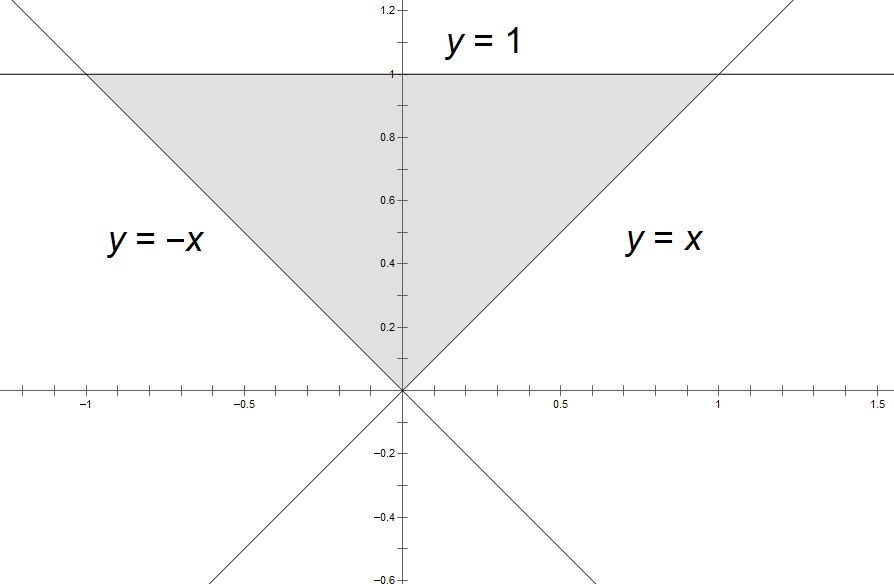
\includegraphics[width=0.3\textwidth]{image/2016数二-题18.png}
\end{figure}

$$
\iint_D{\frac{x^2-xy-y^2}{x^2+y^2}dxdy}=\int_{\frac{\pi}{4}}^{\frac{3\pi}{4}}{d\theta \int_0^{\frac{1}{\sin \theta}}{\frac{r^2\left( \cos ^2\theta -\cos \theta \sin \theta -\sin ^2\theta \right)}{r^2}\cdot rdr}}
$$
$$
=\int_{\frac{\pi}{4}}^{\frac{3\pi}{4}}{d\theta \int_0^{\frac{1}{\sin \theta}}{\left( \cos ^2\theta -\cos \theta \sin \theta -\sin ^2\theta \right) \cdot rdr}}=\int_{\frac{\pi}{4}}^{\frac{3\pi}{4}}{\left( \cos ^2\theta -\cos \theta \sin \theta -\sin ^2\theta \right) \cdot \left. \frac{1}{2}r^2 \right|_{r=0}^{r=\frac{1}{\sin \theta}}d\theta =}
$$
$$
\int_{\frac{\pi}{4}}^{\frac{3\pi}{4}}{\left( \cos ^2\theta -\cos \theta \sin \theta -\sin ^2\theta \right) \cdot \frac{1}{2}\cdot \frac{1}{\sin ^2\theta}d\theta}=\int_{\frac{\pi}{4}}^{\frac{3\pi}{4}}{\left( \cos ^2\theta -\cos \theta \sin \theta -\sin ^2\theta \right) \cdot \frac{1}{2}\cdot \frac{1}{\sin ^2\theta}d\theta}=
$$
$$
\frac{1}{2}\int_{\frac{\pi}{4}}^{\frac{3\pi}{4}}{\cot ^2\theta d\theta -\frac{1}{2}}\int_{\frac{\pi}{4}}^{\frac{3\pi}{4}}{\cot \theta d\theta -\frac{\pi}{4}}
$$
$$
\text{其中}\int_{\frac{\pi}{4}}^{\frac{3\pi}{4}}{\cot ^2\theta d\theta =}\int_{\frac{\pi}{4}}^{\frac{3\pi}{4}}{\csc ^2-1d\theta =}\left( -\cot \theta -\theta \right) _{\theta =\frac{\pi}{4}}^{\theta =\frac{3\pi}{4}}\,\,=\left( -\frac{-\frac{\sqrt{2}}{2}}{\frac{\sqrt{2}}{2}}-\frac{3\pi}{4} \right) -\left( -1-\frac{\pi}{4} \right) =2-\frac{\pi}{2}\text{,}
$$
$$
\int_{\frac{\pi}{4}}^{\frac{3\pi}{4}}{\cot \theta d\theta}=\ln\text{|}\csc \theta -\cot \theta |_{\theta =\frac{\pi}{4}}^{\theta =\frac{3\pi}{4}}=\ln\text{|}-\sqrt{2}+1|-\ln\text{|}\sqrt{2}-1|=0\left( \text{此步也可通过对称性直接算出} \right) \text{,}
$$
$$
\cot ^2\theta +1=\csc ^2\theta ,\left( \cot \theta \right) '=-\csc ^2\theta .
$$
$$
\text{故}\frac{1}{2}\int_{\frac{\pi}{4}}^{\frac{3\pi}{4}}{\cot ^2\theta d\theta -\frac{1}{2}}\int_{\frac{\pi}{4}}^{\frac{3\pi}{4}}{\cot \theta d\theta -\frac{\pi}{4}}=1-\frac{\pi}{4}-\frac{\pi}{4}=1-\frac{\pi}{2}.
$$

\section{}

\subsection{}


\chapter{}

\section{}









\end{document}
